\chapter{Planung}

\section{Vorgehen}

Zuerst muss sich über das Themengebiet informiert werden. Danach erfolgt der
Entwurf eines Konzepts mit daran anschließender Technologieauswahl. Nachdem die
Technologieauswahl getroffen ist wird die notwendige Hardware beschafft und
parallel dazu mit der Aufteilung der Aufgaben in Arbeitspakete begonnen. Im
nächsten Schritt werden die Arbeitspakete in logischer Abfolge abgearbeitet und
das Konzept so schrittweise umgesetzt.

\subsection{Zeitplanung}

Die Zeitplanung ist Semesterbedingt in zwei große Blöcke unterteilt.\\
Im ersten Semester werden folgende Punkte umgesetzt:

\begin{enumerate}
  \item Informationsphase
  \item Entwicklung eines Konzeptes
  \item Technologieauswahl
  \item Beschaffung von notwendiger Hard- und Software
  \item Aufteilung der Aufgaben in Arbeitspakete
  \item Erstellen der Zeitplanung
\end{enumerate}

Im zweiten Semester werden folgende Punkte umgesetzt:

\begin{enumerate}
  \item Abarbeitung der Arbeitspakete
  \item Erstellung der Dokumentation
\end{enumerate}

\subsection{GANTT-Diagramm}

Das folgende GANTT-Diagramm wurde im Rahmen der Zeitplanung erstellt:

\section{Soll-Zustand}
Die Sensoren werden kontinuierlich abgefragt und senden die gemessenen Werte an
die Datenbank auf der Zentraleinheit. Dort werden die Daten entsprechend dem
meldenden Sensorknoten abgespeichert. Die Website greift auf die Datenbank zu
und lädt die Daten in eine tabellarische Darstellung, die der Benutzer dann
sieht. Durch einen Zeitstempel ist es möglich bei Daten der Temperatursensoren
und der Feuchtigkeitssensoren einen Verlauf darzustellen.

\section{Netzplan}

Die Sensoren sind an den Sensorknoten angeschlossen. Die Daten werden per WLAN
an die Zentraleinheit gesendet. Dort werden die Daten in die Datenbank
geschrieben.\\
Der Webserver greift auf die Datenbank zu und stellt die Daten auf einer Website
übersichtlich dar. (\nameref{Darstellung_Umgebung})

\begin{figure} [htb]
\begin{centering}
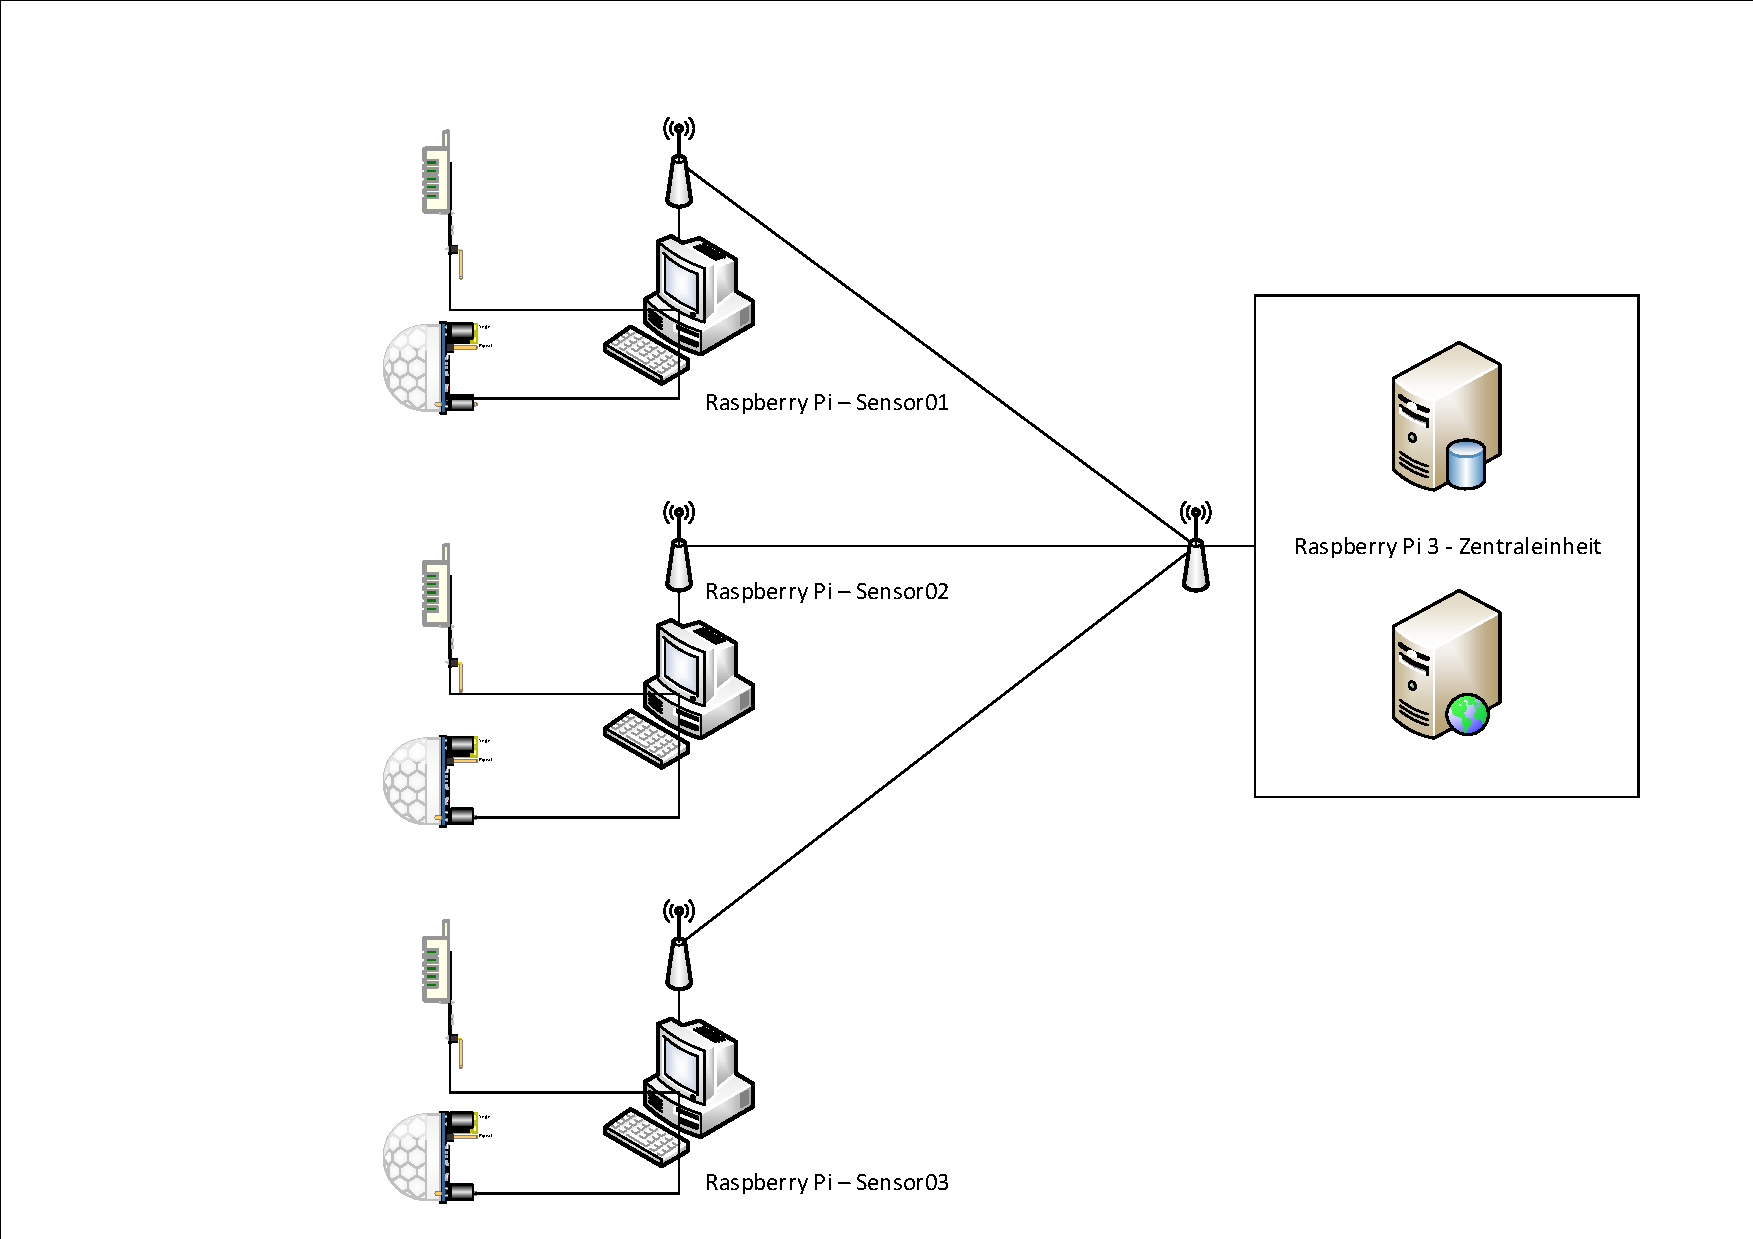
\includegraphics[scale=0.4]{Bilder/Netzplan.pdf}
\caption[Schematische Darstellung der geplanten Umgebung]{Schematische
Darstellung der geplanten Umgebung}
\label{Darstellung_Umgebung}
\end{centering}
\end{figure} 

\section{Datendiagramme}

